\documentclass[
  ukrainian,
  simple,
]{eskdnaukvd}

%%% Font configuration
\setmainfont{STIX Two Text}
\setsansfont{Roboto}
%%%

%%% Math Typesetting
\usepackage{unicode-math}
\setmathfont{STIX Two Math}
%%%

%%% Language configuration
\usepackage{polyglossia}
\setdefaultlanguage{ukrainian}
\setotherlanguage{english}
%%%

%%% List settings
\usepackage{enumitem}
\setlist[enumerate]{
  label*      = {\arabic*.},
  left        = \parindent,
  topsep      = 0\baselineskip,
  parsep      = 0\baselineskip,
  noitemsep, % override itemsep
}
% List settings for levels 2–4
\setlist[enumerate, 2, 3, 4]{
  label*      = {\arabic*.},
  left        = 0em,
  topsep      = 0\baselineskip,
  parsep      = 0\baselineskip,
  noitemsep, % override itemsep
}

\setlist[itemize]{
  label*      = {—},
  left        = \parindent,
  topsep      = 0\baselineskip,
  parsep      = 0\baselineskip,
  itemsep     = 1\baselineskip,
  noitemsep, % override itemsep
}

\setlist[description]{
  font        = {\rmfamily\upshape\bfseries},
  topsep      = 1\baselineskip,
  parsep      = 0\baselineskip,
  itemsep     = 0\baselineskip,
}
%%%

%%% Define width grid
\newlength{\gridunitwidth}
\setlength{\gridunitwidth}{\textwidth / 12}
%%%

%%% GOST strings
\ESKDdepartment{Національний авіаційний університет}
\ESKDclassCode{}
\ESKDtitle{Офісна локальна комп'ютерна мережа}
%\ESKDdocName{Курсова робота}
\ESKDsignature{НАУ 19 2824000 ПЗ}
\ESKDauthor{Клокун~В.\,Д.}
\ESKDtitleApprovedBy{Керівник роботи}{Проценко М.\,М.}
\ESKDchecker{Проценко М.\,М.}
\ESKDcolumnIX{ФККПІ СП-425}
%%%

%%% Define ESKD styles
\ESKDdefaultStyle{nauplain}
%%%

\begin{document}
  \ESKDthisStyle{empty}

  \begin{titlepage}
  \begin{center}
      Міністерство освіти і науки України\\
      Національний авіаційний університет\\
      % Навчально-науковий інститут комп'ютерних інформаційних технологій\\
      Кафедра комп'ютерних систем та мереж

      \vspace{\fill}
      Курсовий проект\\
      (пояснювальна записка)\\

      \vspace{1 \baselineskip}

      студента 4-го курсу\\
      Інституту комп'ютерних інформаційних технологій\\
      Освітньо-кваліфікаційного рівня «Бакалавр»\\
      Напряму підготовки 6.050102 «Комп'ютерна інженерія»

      \vspace{1 \baselineskip}

      \begin{flushleft}
      Тема: офісна локальна комп'ютерна мережа

      \vspace{2 \baselineskip}

      Виконавець: \hfill Клокун В.\,Д.\\
      Керівник: \hfill Проценко М.\,М.
      \end{flushleft}

      \vspace{\fill}

      Київ 2019
    \end{center}
  \end{titlepage}

  \newpage

  % Fix ESKDX page counter to include the title page
  \setcounter{page}{2}
  \section*{Вступ}
  \addcontentsline{toc}{section}{Вступ}
  \ESKDthisStyle{nausection}
    Це текст вступу.

  \section{Технологія «\textenglish{Ethernet}»}
    FIXME.

  \section{Топологія мережі}
  \ESKDthisStyle{nausection}
    Необхідно розробити проект офісної локальної комп'ютерної мережі поставлені такі вимоги для заданого поверху будівлі~(рис.~\ref{fig:floor-plan}).

    \begin{figure}[!htbp]
      \centering
      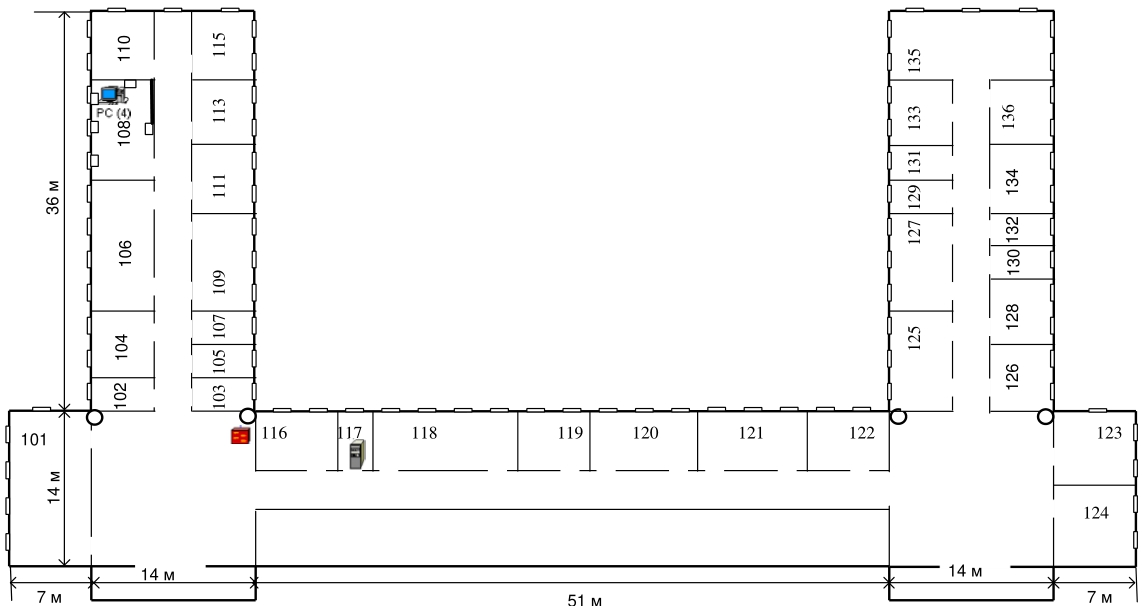
\includegraphics[width = \columnwidth]{./assets/01-floor-plan.jpg}
      \caption{План цільового поверху, для якого необхідно спроектувати локальну комп'ютерну мережу}
      \label{fig:floor-plan}
    \end{figure}

    Також проект має задовольняти мінімальні вимоги до кількості клієнтів~(табл.~\ref{tab:room-clients}), а також вимоги реалізації, а саме:
    \begin{itemize}
      \item серверна кімната має знаходитись в кімнаті~107;
      \item необхідно створити 3 віртуальні локальні мережі~(\textenglish{\allcaps{VLAN}});
      \item розмістити 2~фізичні сервери для накопичення та зберігання даних;
      \item запропонувати рішення щодо встановлення каналу зв'язку з провайдером~\textenglish{Internet}, розподілу~\textenglish{IP}-адрес та трансляції адрес;
      \item передбачити заходи із захисту мережі.
    \end{itemize}
    Розробка проекту починається з вибору топології, і поставлені обмеження дозволяють краще її підібрати.

    \newlength{\tmptabcellwidth}
    \setlength{\tmptabcellwidth}{\columnwidth / 12 - 2 \tabcolsep}
    \begin{table}[!htbp]
      \centering
      \caption{Кімнати та кількість робочих станцій у них}
      \label{tab:room-clients}
      \begin{tabular}{
        |*{12}{b{\tmptabcellwidth}|}
      }
        \hline
          108 & 110 & 109 & 111 & 115 & 118 & 120 & 122 & 125 & 128 & 134 & 136 \\
        \hline
          4 & 3 & 4 & 2 & 2 & 6 & 3 & 3 & 3 & 2 & 2 & 2\\
        \hline
      \end{tabular}
    \end{table}

    \subsection{Вибір топології мережі}

      Враховуючи сформульовані умови і обмеження, топологія, обрана для проектування, має вирішувати такі задачі:
      \begin{itemize}
        \item підтримувати надійність мережі, тобто організувати середовище, в якому несправність одного клієнта якнайменш вплине на інших клієнтів;
        \item сегментувати мережу, тобто розподілити її на менші логічні і структурні одиниці;
        \item задати центральну точку для обміну даними та підключення до інфраструктури провайдера.
      \end{itemize}
      Щоб вирішити такий широкий спектр поставлених задач, для розробки проекту офісної локальної комп'\-ю\-тер\-ної мережі була обрана гібридна топологія~— така топологія, яка поєднує в собі декілька стандартних топологій.

      Щоб задати центральну точку обміну даними та підключення до інфраструктури провайдера, добре підходить топологія~«Зірка»~(рис.~\ref{fig:topology-star}).

      \begin{figure}[!htbp]
        \centering
        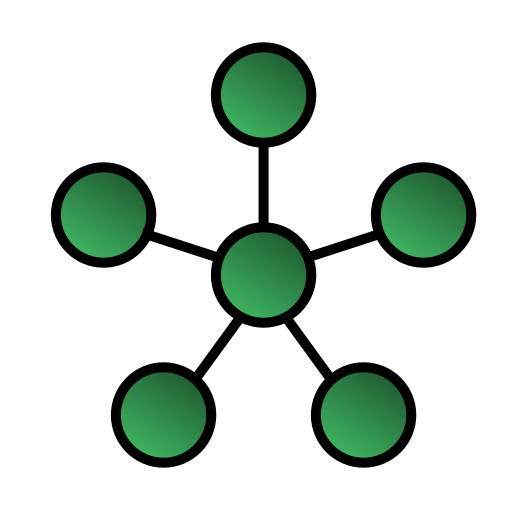
\includegraphics[width = 4 \gridunitwidth]{./assets/02-topology-star.png}
        \caption{Приклад топології~«Зірка»}
        \label{fig:topology-star}
      \end{figure}

      «Зірка» передбачає, що всі точки-клієнти під'єднуються до центральної точки, яка в свою чергу розподіляє і перенаправляє повідомлення між клієнтами або ж повторює повідомлення усім під'єднаним клієнтам. Наявність центральної точки у топології~«Зірка» суттєво збільшує надійність мережі, адже якщо вийде з ладу канал передачі даних між двома точками, лише одна з них буде ізольована від мережі, тобто несправність однієї точки чи каналу обміну даними мінімально вплине на інші клієнти. Однак, топологія «Зірка» має суттєвий недолік~— єдину точку відмови: якщо у топології відмовить центральна точка, вся мережа перестане працювати. Тим не менш, сучасні проектно-технічні засоби на кшталт надійного обладнання, обмеження фізичного доступу та застосування надлишковості дозволяють впоратись з цим недоліком, тому топологія~«Зірка» буде основною структурною одиницею топології розроблюваної мережі.

      Щоб з'єднати структурні сегменти мережі, що проектується, необхідно передбачити можливість підключення усіх існуючих сегментів мережі, а також зручного додавання сегментів у майбутньому. Для цього зручно скласти найменші структурні сегменти в таку ієрархію, в якій найнижчі кінцеві сегменти підключаються до вищих, розподіляючих сегментів, а вищі розподіляючі сегменти~— до ще вищих, і таким чином аж до кореневого вузла доступу, який буде підключений до мережі «Інтернет» через інфраструктуру провайдера.

      Якщо для прикладу розглянути сегменти-«Зірки» як єдиний вузол, такий ієрархічний спосіб під'єднання нагадує топологію «Шина»~(рис.~\ref{fig:topology-bus}), і тому з'єднання сегментів таким способом дозволить підключити усі сегменти одне до одного, а також зручно додавати нові сегменти у майбутньому.

      \begin{figure}[!htbp]
        \centering
        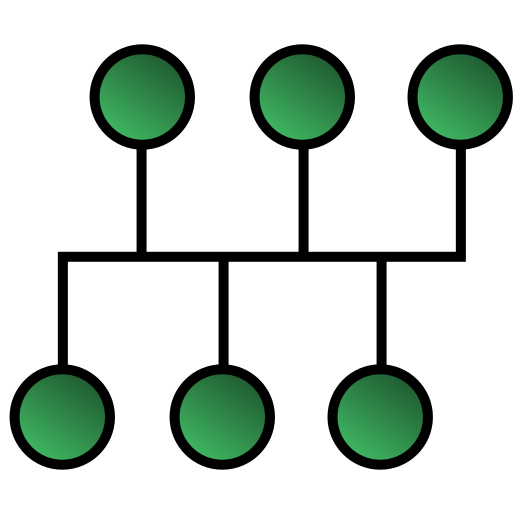
\includegraphics[width = 4 \gridunitwidth]{./assets/03-topology-bus.png}
        \caption{Приклад топології~«Шина»}
        \label{fig:topology-bus}
      \end{figure}

      Отже, необхідна гібридна топологія поєднає у собі властивості стандартних топологій «Зірка» та «Шина». Це поєднання називається деревовидною топологією~(рис.~\ref{fig:tree-topology}).

      Деревовидна топологія є конкретною реалізацією поняття дерева з теорії графів, в якому перший вузол дерева прийнято називати коренем, наступні вузли високих рівнів~— батьками, а низьких рівнів~— дітьми.

      \begin{figure}[!htbp]
        \centering
        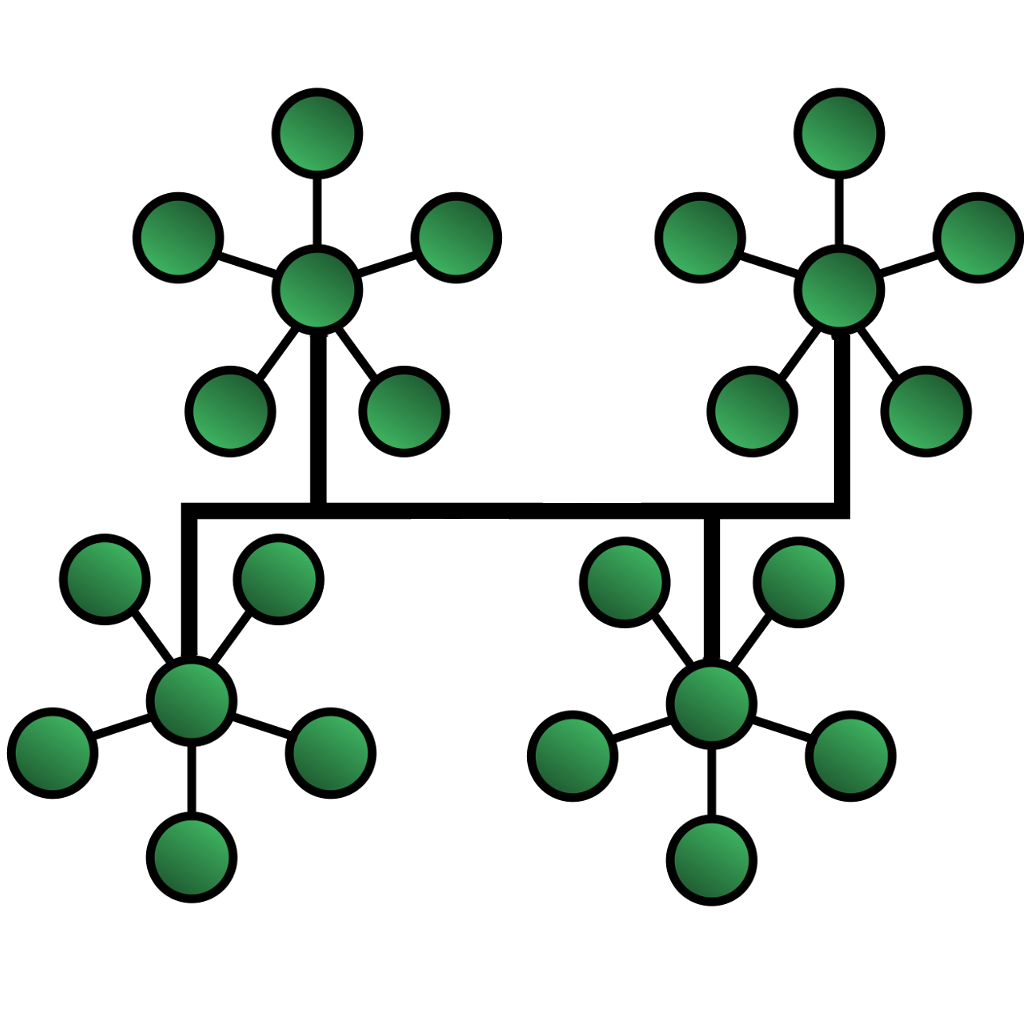
\includegraphics[width = 8 \gridunitwidth]{./assets/04-topology-tree.png}
        \caption{Приклад деревовидної топології}
        \label{fig:tree-topology}
      \end{figure}

      Отже, в результаті вибору була обрана гібридна деревовидна топологія, яка дозволить зручно вирішити задачі і задовольнити вимоги, поставлені до потрібної мережі: забезпечити надійність мережі, сегментувати її, а також організувати центральну точку підключення до провайдера і обміну даними.

    \subsection{Реалізація обраної топології}
      Обравши зручну і ефективну топологію для проекту комп'ютерної мережі, необхідно спроектувати план її втілення. Для цього, перш за все, необхідно скласти перелік обладнання, яке знадобиться для розробки мережі, врахувавши потреби мережі.

      Цільова мережа має підтримувати одночасну роботу не менш ніж 36 робочих станцій різного призначення, а також 2 сервери. Робочі станції повинні бути об'єднані у 3~віртуальні локальні мережі. Щоб задовольнити цю потребу, необхідно використовувати маршрутизатори рівня 2 моделі~\textenglish{\allcaps{OSI}}, які дозволять використати технологію~\textenglish{\allcaps{IEEE}~802.1q}, щоб реалізувати розподіл на віртуальні мережі.

      Враховуючи, що передбачається робота приблизно 36~робочих станцій, а також той факт, що будівля складається з декількох крил, щоб розмістити користувачів у мережі, потребується 2 24-портових комутатори. Також хорошою практикою при реалізації топології є винесення серверів в окрему мережу, що буде реалізовано за допомогою технології віртуальних локальних мереж, але щоб підкреслити можливість розширення мережі і подальше огородити сервери, використаємо для них окремий комутатор. Отже, знадобиться 3 комутатори рівня 2, які будуть комутаторами рівня доступу.

      Оскільки проектована мережа має надавати можливість розширення, підтримувати швидку роботу багатьох робочих станцій з мережею~«Інтернет», а також надавати стабільний і миттєвий доступ до ресурсів двох серверів всередині мережі, доцільно використати пристрій рівня розподілу. Щоб економно організувати високу швидкість обміну даними всередині мережі, варто використати комутатори рівня~3: вони коштують значно дешевше за маршрутизатори аналогічної швидкодії, підтримують всі технології, які можуть знадобитись при організації внутрішньої мережі, а також надають можливість зручного розширення, дозволяючи лише увімкнути новий комутатор рівня~2 і під'єднувати до нього нові клієнти.

      Локальна офісна комп'ютерна мережа, що проектується, передбачає доступ до мережі «Інтернет». Щоб працювати з мережею мережею~«Інтернет», а тим паче від імені 36 клієнтів внутрішньої мережі, необхідно маршрутизувати і перетворювати трафік, який приходить зовні та генерується всередині. Для цього знадобиться маршрутизатор.

      Отже, щоб реалізувати обрану топологію, необхідно таке обладнання:
      \begin{itemize}
        \item Маршрутизатор.
        \item Комутатор рівня 3.
        \item Комутатори рівня 2.
      \end{itemize}
      При реалізації мережі необхідно знати, яке конкретне обладнання варто використовувати, тому необхідно визначити зручні і доцільні конкретні пристрої.

      Так як для моделювання мережі використовується пакет~\textenglish{Cisco Packet Tracer}, то для реалізації мережі буде використане обладнання фірми~\textenglish{Cisco}. Судячи з поставлених вимог, мережа проектується для потреб середнього зростаючого бізнесу, тому будуть розглядатись пристрої саме цієї ніші.

      Отже, для реалізації мережі необхідно 3 24-портових комутатори рівня~2. Серед обладнання, доступного в середовищі~\textenglish{Packet Tracer}, найкраще підходять комутатори~\textenglish{Cisco Catalyst 2960-24TT}, які стануть комутаторами рівня доступу і порти яких будуть розподілені за віртуальними мережами.

      Для організації рівня розподілу досить одного пристрою~— комутатора рівня~3 \textenglish{Cisco Catalyst 3560}, який відповідатиме за об'єднання комутаторів рівня доступу, маршрутизацію трафіка всередині мережі, а також виділення \textenglish{\allcaps{IP}}-адрес клієнтам за протоколом~\textenglish{\allcaps{DHCP}}.

      В рамках задачі доступ до мережі «Інтернет» організується за допомогою інфраструктури провайдера, який надає виділений канал, підключення до якого відбувається за допомогою технології~\textenglish{\allcaps{FTT}x}; термінація на останній милі~— за допомогою витої пари. Враховуючи задані параметри підключення провайдера і проектованої мережі, машрутизатором мережі стане~\textenglish{Cisco Catalyst 2911}, який надає можливість підключення за технологією~\textenglish{Gigabit Ethernet}, а також трансляцію мережевих адрес за допомогою технології~\textenglish{\allcaps{NAT}}. Моделювання інфраструктури провайдера, яка використовується для доступу до мережі «Інтернет», виконуватиметься за допомогою аналогічного маршрутизатора і підключеного до нього публічного сервера.

      Отже, після вибору конкретних пристроїв, була побудована логічна топологія офісної локальної комп'ютерної мережі~(рис.~\ref{fig:net-topology-logical}).

      \begin{figure}[!htbp]
        \centering
        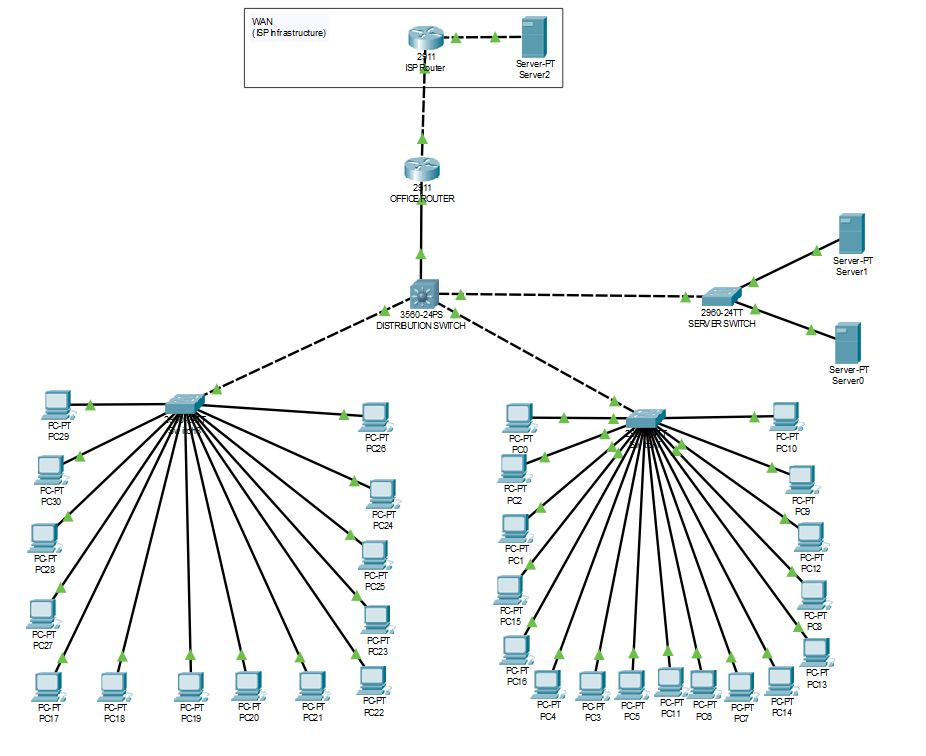
\includegraphics[width = \columnwidth]{./assets/05-net-topology-logical.png}
        \caption{Реалізація логічної топології для проектованої офісної мережі}
        \label{fig:net-topology-logical}
      \end{figure}

      Розглянемо призначення складових топології детальніше.

      \begin{table}[!htbp]
        \centering
        \caption{}
        \label{}
        \begin{tabular}{
          |v{3 \gridunitwidth - 2 \tabcolsep}
          |v{3 \gridunitwidth - 2 \tabcolsep}
          |v{6 \gridunitwidth - 2 \tabcolsep}
          |
        }
          \hline
            Пристрій & \textenglish{\allcaps{VLAN}} & Призначення \\
          \hline
          \hline
        \end{tabular}
      \end{table}

  \section{Налаштування мережі}
  \ESKDthisStyle{nausection}
\end{document}
